\documentclass[
  11pt,
  letterpaper,
   addpoints,
   %answers
  ]{exam}

\usepackage{../exercise-preamble}

\begin{document}

\noindent
\begin{minipage}{0.47\textwidth}

\includegraphics[width=\textwidth]{../fcfm_die}
\end{minipage}
\begin{minipage}{0.53\textwidth}
\begin{center} 
\large\textbf{Fundamentos de control de sistemas} (EL4111-1) \\
\large\textbf{Pauta control 1} \\
\small Prof.~Roberto Cardenas Dobson\\
\small Prof.~Aux.~Osvaldo Jimenez - Erik Sáez\\
\small Ayudantes.~Simon Arenas- Juan Pablo Baez - Francisco Garces - Sofia Ibarra\\
\end{center}
\end{minipage}

\vspace{0.5cm}
\noindent
\vspace{.85cm}

\begin{questions}
    %%%%%%%%%%%%%%%%%%%%%%%%%%%
    \question Teniendo la siguiente planta:
    \begin{align}
        G_p(s) = \frac{1,429 - s}{(s + 1,429)(s^2 + s + 1)} \tag{1}
    \end{align}
    
    El diseño de control a lazo cerrado debe cumplir con las siguientes especificaciones:
    \begin{enumerate}
        \item Máximo sobrepaso = 4.3254\%
        \item Frecuencia natural = 0.722
        \item Cero error en estado estacionario a entrada escalón.
    \end{enumerate}
    
    Se pide lo siguiente:
    \begin{enumerate}
        \item[(a)] Utilizando las condiciones de módulo y ángulo, diseñe un controlador bipropio que cumpla con las especificaciones mencionadas. Utilice cancelación en su diseño si lo considera necesario. (20/50)
        \item[(b)] El ingeniero a cargo del proyecto se da cuenta de que debe considerar los límites físicos de la planta para diseñar correctamente el controlador. Modifique su controlador para que incluya anti-windup generalizado (determine el diagrama de control). De no ser posible aplicar este esquema, explique por qué y proponga otro esquema de anti-windup. (10/50)
        \item[(c)] Por un error de implementación, la ganancia del controlador diseñado en (a) aumenta en un 100\%. ¿Todavía existe cero error de estado estacionario bajo esta nueva condición o ya no es posible lograr este objetivo dado el error de implementación cometido? Fundamente adecuadamente su respuesta. (10/50)
        \item[(d)] Suponga que ahora debe rediseñar el controlador propuesto en (a), con el propósito de que se permita alcanzar cero error en estado estacionario a una entrada de la forma \(e(t) = A_m t^2 + B_m \sin(\omega_1 t) + C_m \cos(\omega_2 t)\). ¿Cuáles son los elementos mínimos que debe tener la función de transferencia de este controlador para cumplir con estos requerimientos? Proponga una expresión para el controlador que cumpliría con estos requisitos. (10/50)\\
    \end{enumerate}
%----------------------------------
\begin{solution}
    \subsection*{Resolucion a)}
    Tenemos que el maximo paso de sobrepaso viene dado por MOV = 4.3254\%, ademas dadA la frecuencia natural, $w_n = 0.722$, podemos obtener el valor de $\xi$ , el cual vendra dado por:
    \begin{align}
        e^{\frac{-\xi \pi}{\sqrt{1-\xi^{2}}}} &= 0.043219\\
        \frac{-\xi \pi}{\sqrt{1-\xi1^{2}}} &= ln(0.04321)\\
        \xi &= 0.707
    \end{align}
    Luego tenemos que el punto de diseño:
    \begin{align}
        s_{1,2} = -\xi w_n \pm jw_n\sqrt{1-\xi^{2}} = -0.5105 \pm j0.5105
    \end{align}
    Tenemos que  la planta al factorizar el denominador de la planta esta vendra dada por :
    \begin{align}
        G_{p}(s) = \frac{(1.429 - s)}{(s+1.429)\left(s + \frac{1}{2} + j\frac{\sqrt{3}}{2}\right)\left(s+ \frac{1}{2} - \frac{\sqrt{3}}{2}\right)}
    \end{align}
    Es importante destacar, que la ganancia con la que evaluaremos el sistema sera negativa, debido a la forma del numerador (\textit{Notar que lo que esta presente es la aproximacion de Pade del retardo}). Luego como se permite el aplicar cancelacion el controlador sera por tanto:
    \begin{align}
        G_{c}(s) = K \frac{\left(s + \frac{1}{2} + j\frac{\sqrt{3}}{2}\right)\left(s+ \frac{1}{2} - \frac{\sqrt{3}}{2}\right)}{s(s+a)}
    \end{align}
    De esta manera tenemos que con el integrador (1/s) es posible el obtener cero error a estado estacionario y con (s+a) nos permite sintonizar el controlador para el punto de diseño. Luego el LGR vendra dado por:
    \begin{center}
        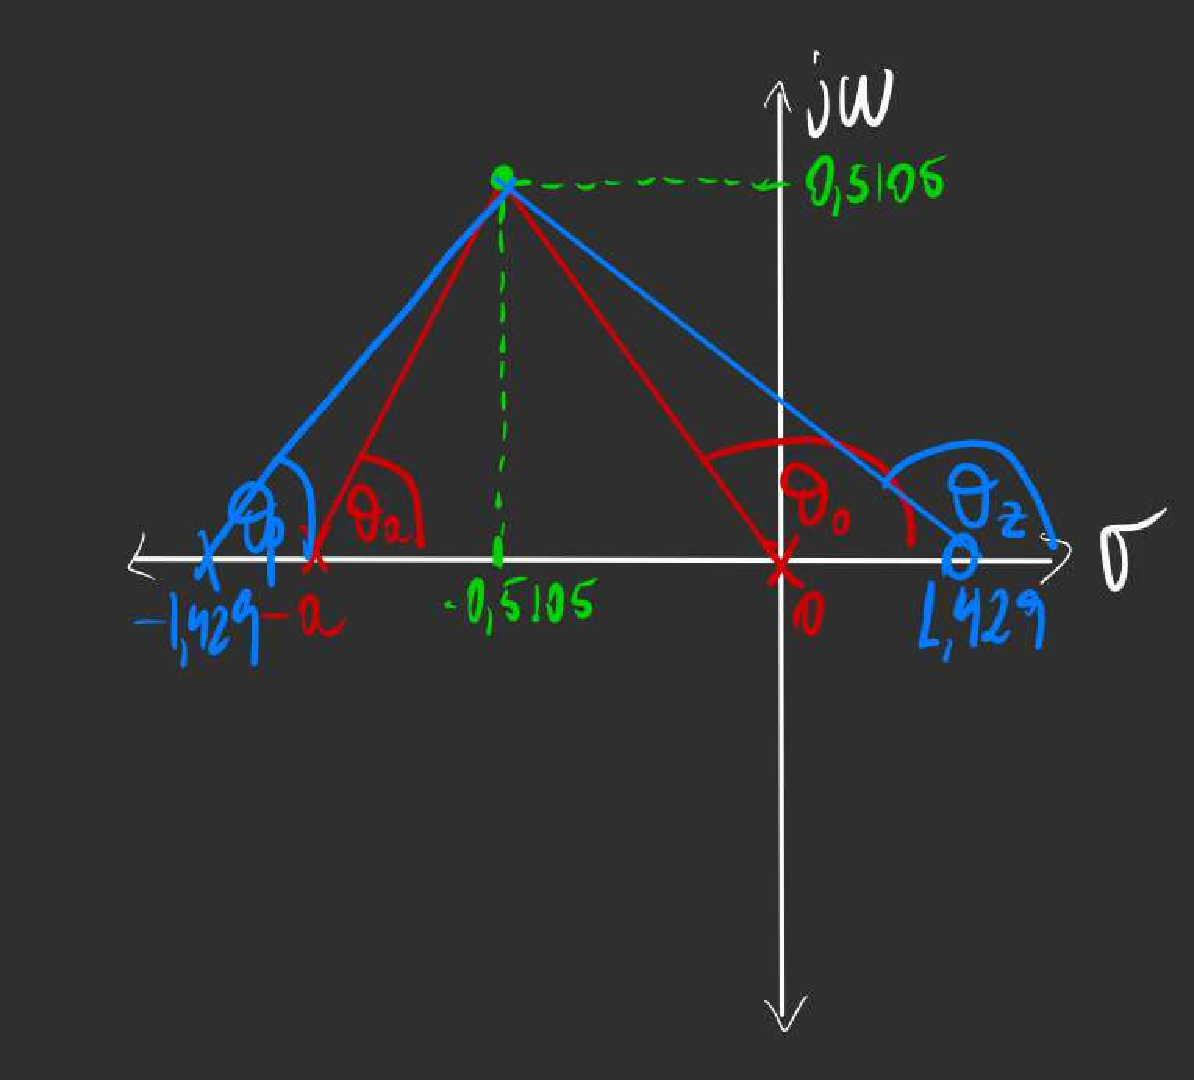
\includegraphics[width=0.35\textwidth]{Control_P1_1}
        \captionof{figure}{LGR del sistema de lazo cerrado} 
      \end{center}
    Como se menciono anteriormente la ganancia sera negativa, eso implica que:
    \begin{align}
        \sum_{i=1}^{n} \theta_{p_{i}} - \sum_{i=1}^{m} \theta_{z_{i}} = 0^{\circ} 
    \end{align}
    Con lo que para todos angulos se tiene:
    \begin{align}
        \theta_o &= 180^{\circ} - \tan^{-1}\left(\frac{0.5105}{0.5105}\right) = 135^{\circ} \\
        \theta_z &= 180^{\circ} - \tan^{-1}\left(\frac{0.5105}{0.5105 + 1.429}\right) = 165.25^{\circ} \\
        \theta_a &= \tan^{-1}\left( \frac{0.5105}{a - 0.05105}\right) \\
        \theta_p &= \tan^{-1}\left( \frac{0.5105}{1.429 - 0.5105}\right) = 29.07^{\circ}
    \end{align}
    Retomando la condicion de angulo se obtiene que:
    \begin{align}
        \theta_p + \theta_0 + \theta_a - \theta_z &= 0\\
        \theta_{a}&=\tan(1.18^{\circ})
    \end{align}
    De esta manera se obtiene que el punto a en el eje real, vendra dado por:
    \begin{align}
        a &=25.27
    \end{align}
    Una vez obtenido el punto a, es posible calcular la ganancia la cual viene dada por:
    \begin{align}
        K &= \frac{1}{|G_{p}(s)G_{c}(s)|}_{s^{*}}\\
        &=9.3758
    \end{align}
    Con lo que el controlador vendra dado por:
    \begin{align}
        G_{c}(s) = 9.3758 \frac{\left(s + \frac{1}{2} + j\frac{\sqrt{3}}{2}\right)\left(s+ \frac{1}{2} - \frac{\sqrt{3}}{2}\right)}{s(s+25.27)}
    \end{align}
    \subsection*{Resolucion b)}
    Se consideran los limites fisicos de la planta, por lo que es necesario aplicar anti-windup generalizado, el cual vendra dado por:
    \begin{align}
        K_{\infty} &= \lim_{s \to \infty} 
            G_{c}(s) = lim_{s \to \infty} \left(9.3758 \frac{\left(s + \frac{1}{2} + j\frac{\sqrt{3}}{2}\right)\left(s+ \frac{1}{2} - \frac{\sqrt{3}}{2}\right)}{s(s+25.27)}\right)
        = 9.3758
    \end{align}
Por ultimo tenemos que
\begin{align}
    K^{-1} = \frac{1}{9.3758} \cdot \frac{s^{2} + 25.29s}{s^{2}+s +1}
\end{align}
Con lo que el ultimo bloque vendra dado por:
\begin{align}
    K^{-1} - K_{\infty}^{-1} = \frac{1}{9.3758} \cdot \left(\frac{24.29s-1}{s^{2}+s+1}\right)
\end{align}
Con lo que el esquema de antiwindup vendra dado por:
\begin{center}
    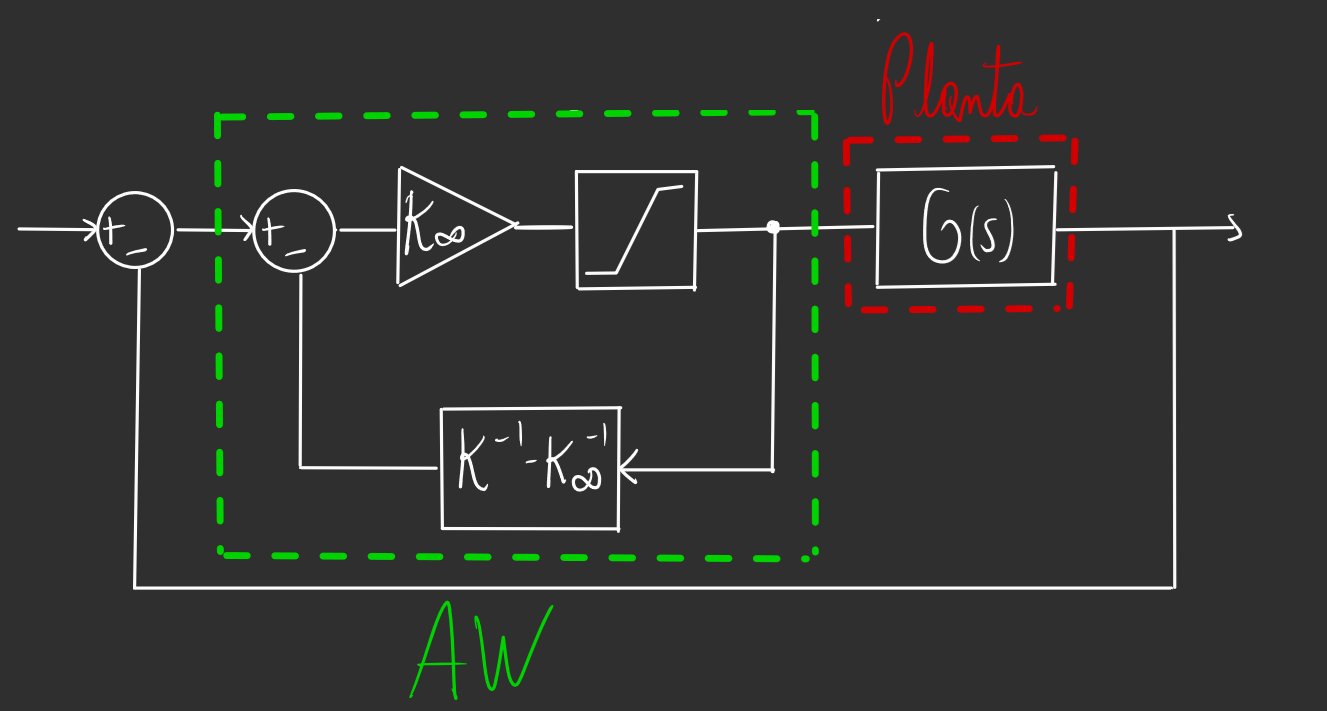
\includegraphics[width=0.4\textwidth]{Control_P1_2.png}
    \captionof{figure}{Esquema de anti-windup generalizado} 
  \end{center}
\subsection*{Resolucion c)}
Se busca obtener el cero error a estado estacionario cuando la ganancia aumenta en un 100\%.De antemano se tiene que el error a estado estacionario no se ve afectado por la genencia debido a que:
\begin{align}
    \hat{e}= \lim_{s \to 0} sE(s) = \lim_{s \to 0} \left(\frac{s \cdot \frac{1}{s}}{1+ \frac{s-1.429}{s(s+25.29)(s+1.429)}}\right) = 0
\end{align}
Por lo que se mantendra el cero error a estado estacionario, pero se debe tener el cuidado con valores de ganancia que produzcan inestabilidad (\textit{Este sistema es estable para $\hat{k} = 2k$ que es un aumento del 100\%})
\subsection*{Resolucion d)}
Sea una entrada $u(t)= A_m t^{2} + B_m sin(w_{1}t) + C_m cos(w_{2}t)$, por lo que se debe tener un controlador que permita el cero error a estado estacionario. Aplicando la transformada de Laplace:
\begin{align}
    L\{u(t)\} = \frac{2A_m}{s^{3}} + \frac{B_m \omega_{1}}{s^{2} + \omega_{1}^{2}} + \frac{C_m \omega_{2}}{s^{2} + \omega_{2}^{2}}
\end{align}
Luego nos interesa unicamente el denominador, el cual viene dado por:
\begin{align}
    s^{3}(s^{2}+w_{1}^{2})(s^{2} + w_{2}^{2})
\end{align}
Con lo que el controlador debe poseer dicho termino en su denominador, por tanto:
\begin{align}
    G_{c}(s) = k \frac{\Pi (s+ z_{i}) }{ s^{3}(s^{2}+w_{1}^{2})(s^{2} + w_{2}^{2})}
\end{align}

\end{solution}
%----------------------------------
    \question 
    \begin{itemize}
        \item[(a)] Se tiene un sistema en lazo abierto, con realimentación unitaria, que tiene la siguiente función de transferencia:
        \begin{align}
            G(s) = \frac{s + 6}{(s - 3)(s - 4)}
        \end{align}
        \begin{enumerate}
            \item Para un proporcional encuentre, utilizando LGR o Routh-Hurwitz, la zona de ganancias donde el sistema es estable. (10/50)
            \item Si se quiere operar con polos reales y con la máxima frecuencia natural posible en el/los polos dominantes, ¿Cuál debería ser la ganancia en un controlador proporcional? Fundamente su respuesta. (10/50)
        \end{enumerate}
        \item[(b)] Para el sistema de lazos anidados que se encuentra a continuación se pide (asuma \(y(s)^*\) como entrada escalón):
        \begin{figure}[h!]
            \centering
            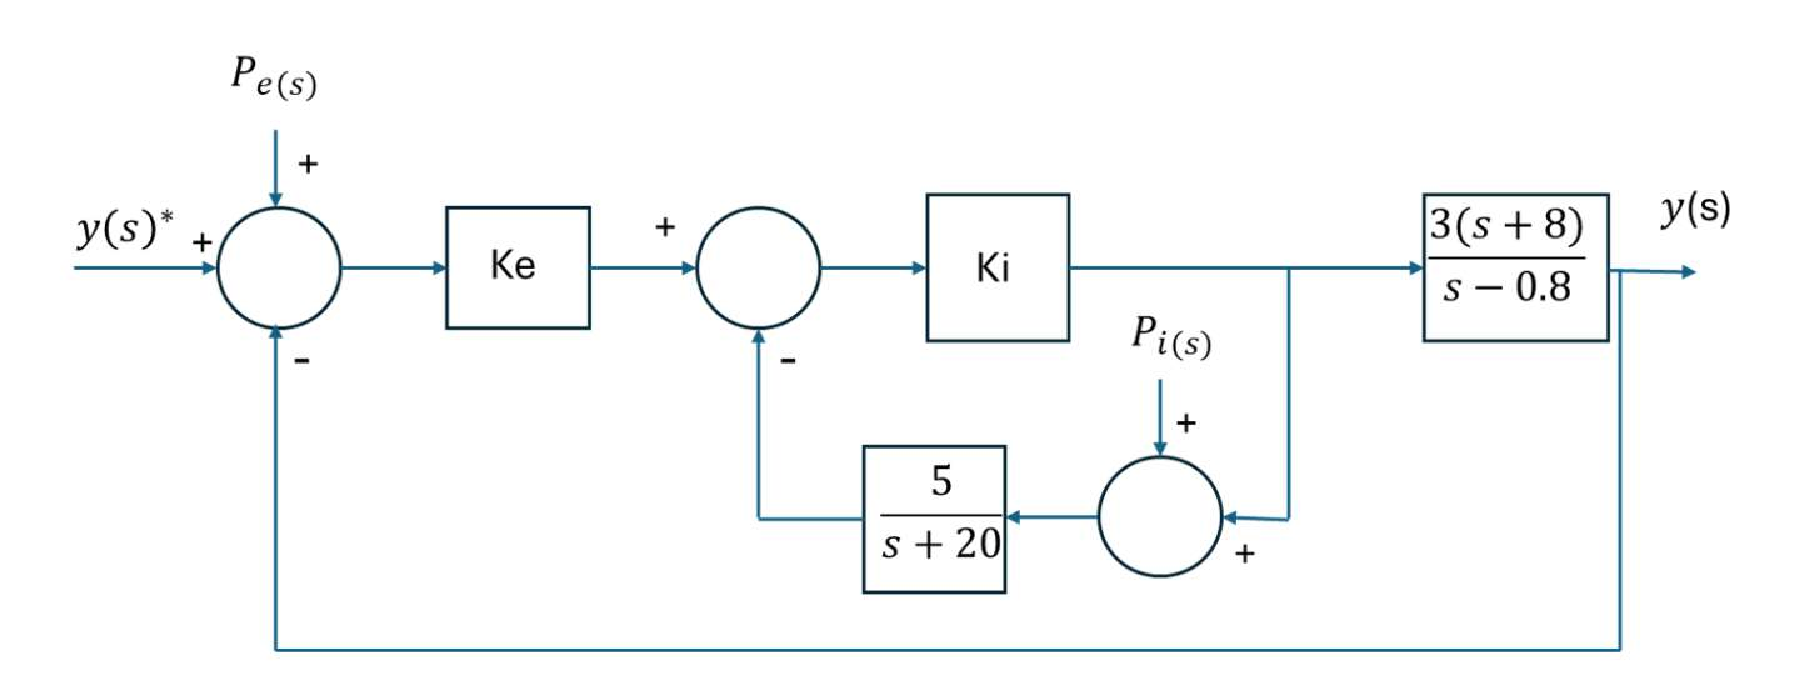
\includegraphics[width=0.7\textwidth]{Control_P2}
        \end{figure}
        \begin{enumerate}
            \item[(1)] Utilizando \(K_i = 2\), se debe diseñar el lazo externo. Elija un coeficiente de amortiguamiento adecuado y, utilizando LGR, encuentre el controlador proporcional necesario para obtener una frecuencia natural de \(\omega_n = 3.5 \, \text{rad/seg}\). (10/50)
            \item[(2)] Existen dos perturbaciones en el sistema, \(P_e(s)\) y \(P_i(s)\). ¿Cuál de estas perturbaciones tiene mayor probabilidad de producir inestabilidad asintótica en el sistema de lazos anidados? Fundamente su respuesta. (10/50)
            \item[(3)] Por envejecimiento, la ganancia \(K_i\) disminuye a un décimo del valor original. El sistema diseñado en b.1 ¿sigue siendo asintóticamente estable en ese caso? Fundamente su respuesta. (10/50)
        \end{enumerate}
    \end{itemize}
    
%------------------------
\begin{solution}
\subsection*{Resolucion a)-1)}
Primero se dibuja el LGR de la planta
\begin{center}
    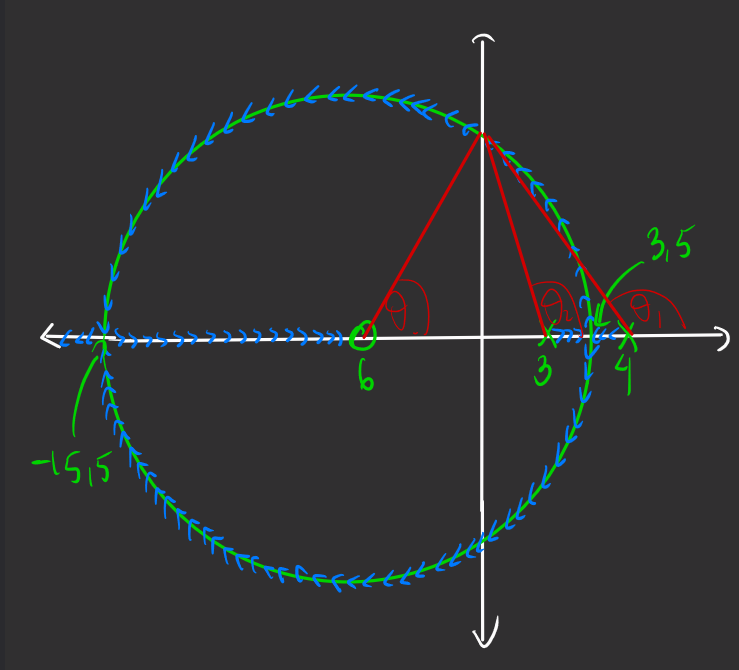
\includegraphics[width=0.4\textwidth]{Control_P1_3.png}
    \captionof{figure}{LGR del sistema de lazo cerrado} 
\end{center}
Los puntos de arranque vienen dados:
\begin{align}
    1+K(s)G(s) &= 0\\
    K(s) = \frac{-(s^{2}-7s+12)}{(s+6)}
\end{align}
Luego aplicando la derivada tenemos que:
\begin{align}
    \frac{\partial K(s)}{\partial s} &= \frac{-(2s+7)(s+6)+s^{2}-7s+12}{(s+6)^{2}}=0\\
    s_{1,2} &= -6 \pm 9.5
\end{align}
Con lo que se obtiene dos puntos, uno asociado a la llegada y otro a la salida, siendo:
\begin{align}
    s_{1}(Salida) &= 3.5\\
    s_{2}(llegada) &= -15.5
\end{align}
Una primera forma para obtener la ganancia critica viene dada por s=jw, es decir en el corte, por tanto:
\begin{align}
    1+ \frac{k(s+6)}{(s-3)(s-4)}&=0\\
    s^{2}-7s +12 +k(s+6)&=0\\
    (jw)^{2} -7(jw) + 12 + k(jw+6) &=0\\
    -w^{2} +12 +6k + j(kw-7w) &=0
\end{align}
Con lo que igualando tanto parte real como compleja a 0, tenemos que:
\begin{align}
    w &= \pm 7.3485\\
    k &= 7
\end{align}
Luego para valores de k<7 el sistema es inestable. De igual manera se puede hacer por R-H:
\begin{align}
    s^{2} -7s +12 + k(s+6) &=0\\
    s^{2} s(k+7) +6k+12 &= 0
\end{align} 
Se tendra que la tabla viene dada por:
\begin{center}
    \begin{tabular}{|c|cc|}
        \hline
        $s^{2}$ & 1 & 6k+12\\
        $s^{1}$ & k-7 & 0\\
        $s^{0}$ & 6k+12 & 0\\
        \hline
    \end{tabular}
\end{center}
Con lo que impeniendo la condiciones estabilidad tenemos que:
\begin{align}
    k-7 > 0    \Rightarrow& k>7 \\
    6k+12 > 0  \Rightarrow& k>-2
\end{align}
Luego tenemos que para $k > 7$ el sistema es estable.
\subsection*{Resolucion a) - 2)}
Luego dado que el punto de llegada esta ubicado en -15.5, luego los polos ubicados en ese punto tendran la frecuencia maxima, por lo tanto tenemos que su ganancia vendra dado por:
\begin{align}
    K= \frac{\Pi \text{Distancia polos}}{\Pi \text{Distancia ceros}} = \frac{(15.5+3)(15.5+4)}{15.5-6} = 37.974
\end{align}
De manera grafica se tiene que:
\begin{center}
    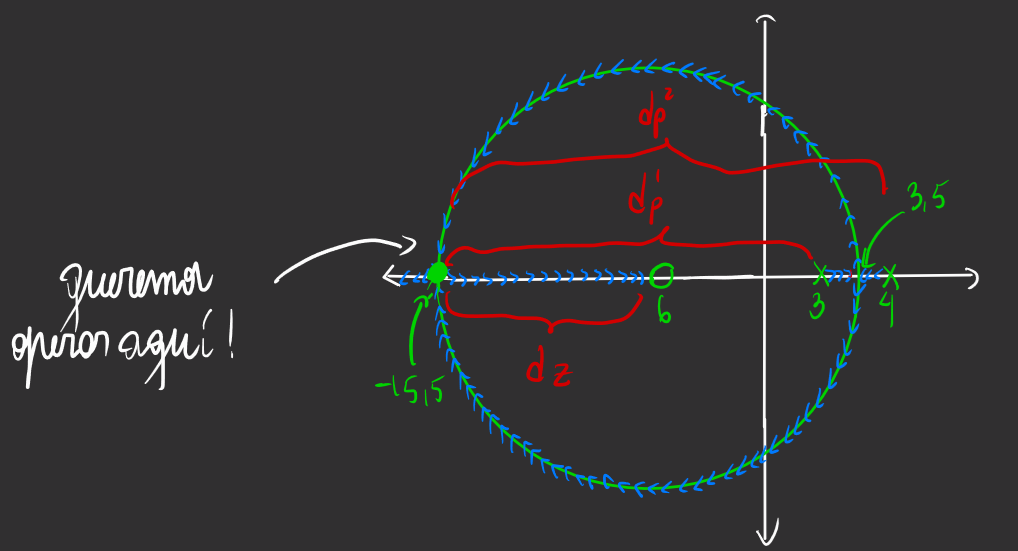
\includegraphics[width=0.45\textwidth]{Control_P1_4.png}
    \captionof{figure}{LGR del sistema de lazo cerrado} 
\end{center}
\subsection*{Resolucion b) - 1)}
Luego tenemos el siguiente para el lazo externo:
\begin{center}
    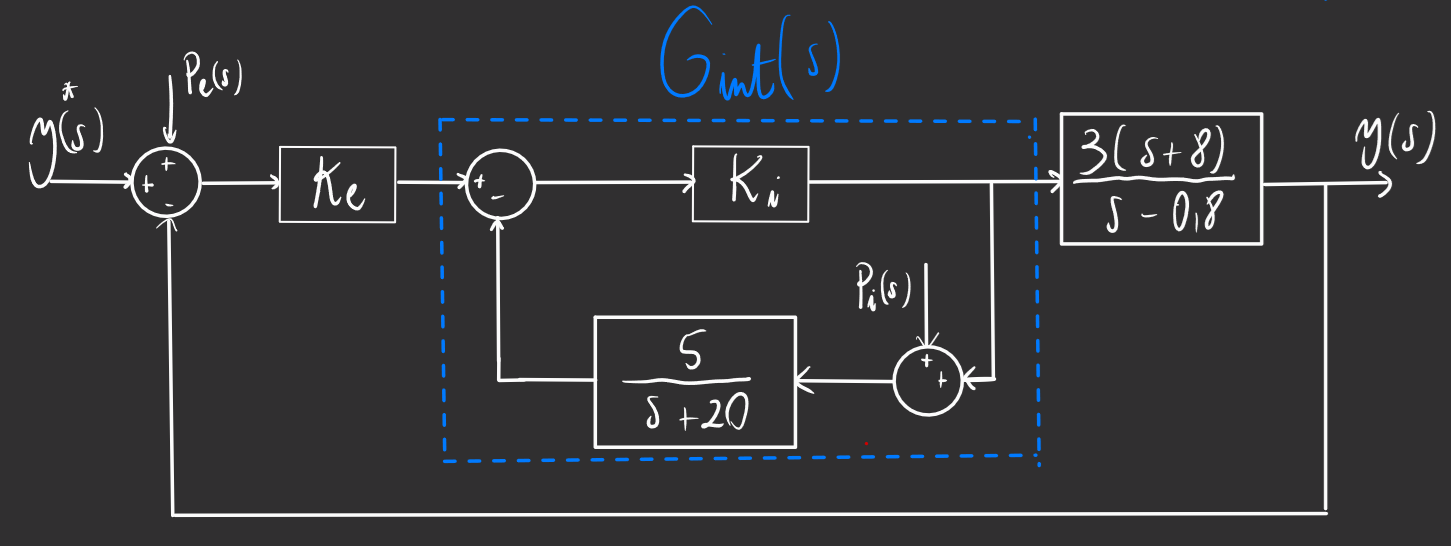
\includegraphics[width=0.6\textwidth]{Control_P1_5.png}
    \captionof{figure}{Esquema del lazo interno} 
\end{center}
\begin{align}
    G_{int}(s) = \frac{K_{i}}{1+\frac{5K_i}{s+20}}= \frac{2(s+20)}{s+30}
\end{align}
Luego aplicando el teorema de valor final a una entrada escalon tenemos que:
\begin{align}
    lim_{s \rightarrow 0}\left(\frac{s \cdot \frac{1}{s}}{1+ \frac{5K_i}{(s+20)}}\right) = lim_{s \rightarrow 0} \left(\frac{k_{i}(s+20)}{s+20+5k_i}\right) = \frac{20}{30} = \frac{2}{3}
\end{align}
Luego diseñando el lazo externo se tiene qu e, dado que el LGR corresponde a un polo y un cero, se tendra que necesariamente $\xi=1$, dado que el LGR se encuentra solo en la parte real. Luego se tiene que:
\begin{align}
    s_{1,2}^{*} = -3.5 \cdot 1 \pm j3.5 \cdot \sqrt{1-1^{2}} = -3.5 \pm j0 = -3.5
\end{align}
Con lo que la ganancia mediante condicion de modulo:
\begin{align}
    K_{e} = \left| \frac{1}{\frac{2(s+8)}{s-0.8}}\right|_{s=-3.5} = 0.477
\end{align}
\subsection*{2) - b)}
Tenemos que las pertubacion no afectan a la estabilidad asintotica.
\subsection*{2) - c)}
Graficamente , la ganancia sistematica critica estara dada por:
\begin{align}
    K^{*}_{sys} = \frac{0.8}{8} = 0.1  
\end{align}
Con lo que se tiene que :
\begin{align}
    K_{sys} = k_{e} \cdot \frac{2}{3} \cdot 3 = 2k_{e}
\end{align}
Finalmente , $k^{*}_{e} =\frac{k^{*}_{sys}}{2} = \frac{0.1}{2} = 0.05$, lo que implica que la inestabilidad vendra dad para $k<0.05$, luego si $k_{e} = 0.04777$, entonces el sistema deja de ser asintoticamente estable.
\end{solution}
%-----------------------


\end{questions}
\newpage
%%%%%%%%%%%%%%%%%%%%%%%%%%%

\end{document}